\chapter{Optimizations of NAS Algorithm}
\label{chap:nas_optimizations}

\begin{sloppypar}
While black-box Neural Architecture Search (NAS), as described in the Section~\ref{chap:nas}, offers a highly flexible and effective framework for discovering high-performing models, it is also notoriously resource-intensive and time-consuming. These limitations make it challenging to apply in real-world scenarios, particularly on constrained hardware as many discovered models will not be compatible to some microcontrollers. 
In this chapter, we present a set of optimization strategies aimed at enhancing the efficiency of black-box neural architecture search (NAS), with a particular focus on accelerating model evaluations and reducing overall search time—while maintaining the quality of the resulting architectures.
\end{sloppypar}

\section{Memory Estimation}

As previously discussed, one of the most significant challenges in this work was designing neural network architectures that fit within the strict memory constraints of the Arduino deployment environment. Initially, the process involved generating an architecture, training it, and attempting deployment—only to discover that the model exceeded the hardware limitations. 

This trial-and-error approach proved inefficient and was quickly abandoned. To address this, we developed a memory estimation mechanism capable of predicting the resource consumption of a model based solely on its architectural configuration. This allowed us to pre-screen candidate models and discard those unlikely to meet the deployment constraints, thereby accelerating the NAS process and conserving computational resources.

In addition, based on these memory estimations, we were able to predict secondary metrics such as inference time and energy consumption—values that previously required the model to be deployed in order to be measured. This advancement further streamlined the design and evaluation process.


To successfully deploy our neural network on the Arduino Nano 33 BLE Sense, we must account for the device’s limited usable memory resources—approximately 256KB of RAM and 1MB of Flash, though a portion of this is reserved for system operations, runtime overhead, and supporting libraries. As a result, the effective memory available for model deployment is lower than the hardware maximum. Any model that exceeds these practical limits is considered undeployable, regardless of its theoretical accuracy or performance.

While the most accurate way to measure memory usage is by compiling and deploying each model onto the microcontroller to observe its actual runtime behavior, this process is highly time-consuming and significantly reduces the number of models that can be evaluated within a given time frame. This is particularly, impractical when evaluating thousands of candidate architectures during Neural Architecture Search (NAS). Consequently, there is a critical need for fast and reliable approximation methods capable of predicting RAM and Flash consumption without requiring actual deployment.


Based on prior research \cite{tensorflow_RamEstimation}, \cite{liberis2019neural} , we make reasonable assumptions to model
memory consumption:

• RAM usage is estimated by analyzing activation tensor sizes during inference, considering their lifetimes and potential coexistence.

• Flash usage is initially approximated from the number of model parameters, then
corrected using a regression model to account for format overheads like quantization
metadata and FlatBuffer structure.

These assumptions allow us to perform fast memory estimations with reasonable accuracy, enabling effective filtering and prioritization of architectures before committing to
the costly deployment step. To improve the quality of these estimates, empirical data
was collected and regression models were trained to correct for systematic biases in the naive estimators. The resulting tools are embedded in the module, ensuring that only
deployable models are selected for further optimization

To fully understand the capabilities and resource limitations of our device, we conducted experimental analysis to identify the sources of memory overhead. This overhead arises from several essential components required for model execution and embedded functionality:

\begin{itemize}
    \item \textbf{Flash Memory Overhead:} In addition to the model weights and logic—stored in a \texttt{.h} file converted from a \texttt{.tflite} model and consuming the majority of board's memory, additional consumption arises from:
    \begin{itemize}
    
        \item \textbf{CMSIS-NN / Inference Functions:} Optimized functions responsible for executing the neural network layers (e.g., \texttt{arm\_nn\_softmax\_common}, \texttt{arm\_depthwise\_conv\_opt}, etc.) are stored in Flash memory. The more complex the model (i.e., more layers or operations), the more Flash these functions consume.
        
        \item \textbf{Arduino Sketch Code:} To deploy the model on the board, a sketch is used that includes constant variables, initialized pointers, additional libraries, static variables, and runtime logic. 

        \item \textbf{Embedded Input Data:} Input data used for testing (e.g., sample images) is stored as \texttt{const} arrays in Flash. While this contributes to Flash consumption, it avoids any additional RAM usage beyond the input tensor buffer already managed by the inference engine.

    \end{itemize}
\end{itemize}

\bigskip

\begin{itemize}
    \item \textbf{RAM Overhead:} Beyond the Tensor Arena—which is allocated specifically for intermediate buffers during inference—several other components consume RAM:
    \begin{itemize}
        \item \textbf{Main Stack} (\textasciitilde32~KB): Reserved for function calls, local variables, and handling interrupts. This ensures safe execution across diverse runtime scenarios.
        \item \textbf{Standard Library Buffers:}
        \begin{itemize}
            \item \texttt{impure\_data} (\textasciitilde2~KB) and \texttt{\_\_malloc\_av\_} (\textasciitilde41~KB): Internal allocations used by the newlib C library for dynamic memory and standard I/O handling.
        \end{itemize}
        \item \textbf{System Threads and OS Buffers:}
        \begin{itemize}
            \item \texttt{os\_timer\_thread\_stack}: Allocated for RTOS timer handling and related system threads.
        \end{itemize}
        \item \textbf{Peripheral and Communication Buffers:}
        \begin{itemize}
            \item Buffers used by \texttt{\_SerialUSB}, I2C interfaces (\texttt{Wire}, \texttt{Wire1}), and other hardware drivers consume variable RAM depending on their initialization.
        \end{itemize}
        \item \textbf{Static Objects and Runtime Metadata:}
        \begin{itemize}
            \item Instances like \texttt{\_ZZ5setupE8resolver} and static variables declared in the sketch occupy RAM during execution.
        \end{itemize}
        \item \textbf{Interrupt Handlers and Background Tasks:} RAM is also consumed by interrupt service routines (e.g., for BLE events, sensor data polling) and background OS tasks.
    \end{itemize}
\end{itemize}


Empirical measurements during deployment revealed that, in addition to the model's footprint, the following are typical overheads:

\begin{itemize}

    \item \textbf{Flash Usage:} Approximately 200--210~KB, depending on model complexity, the size of embedded data (e.g., input arrays), and the libraries included in the compiled sketch.
    
    \item \textbf{RAM Overhead:} Approximately 45--50~KB is consumed by system components, including the main stack, standard library buffers, RTOS threads, communication drivers, and runtime metadata. The remaining RAM is available for the Tensor Arena used by TensorFlow Lite Micro.

\end{itemize}








\subsection{Flash Memory Estimation}
\label{subsec:flash_memory_estimation}
Estimating the amount of flash memory needed to deploy a neural network model on a microcontroller is a crucial step in the development of edge computing applications, especially in environments where resources such as memory and processing power are severely limited. Flash memory, typically used as read-only memory (ROM), must store the model's parameters, which include the weights and biases of the neural network. These parameters define the behavior of the model and are essential for its operation during inference. A widely used method to estimate the flash memory requirement is to calculate the total storage needed for all the model's parameters. This involves summing up the memory footprint of each weight and bias, which are usually represented as floating-point or fixed-point numbers. By understanding the total number of parameters and their respective data types, developers can make an informed estimate of the memory space required for storing the model on a microcontroller. \cite{pau2023tiny}.

This method is fast and easy to compute, but it doesn't accurately reflect the size of a fully converted \texttt{.tflite} model due to additional overhead such as:
\begin{itemize}
    \item Quantization calibration parameters
    \item Padding and alignment used in FlatBuffer format \cite{manor2022custom}
\end{itemize}



The initial estimation function used the following logic:
\[
\text{Estimated Flash (KB)} = \frac{\text{Total Parameters} \times \text{Data Type Size (Bytes)}}{1024}
\]

This approach uses the \texttt{count\_params()} method from Keras and assumes a constant multiplier depending on data type. In our case, we have quantized the model, our datatype is int8 (1 byte).

While efficient, this method consistently underestimates the actual TFLite model size, which might allow bigger than the allowed to be trained while it will not fit in the deployment enviroment making it time consuming training something too big.

To verify accuracy, a dataset of real models was collected. Each model was:
\begin{enumerate}
    \item Built using Keras
    \item Converted to TFLite with full integer quantization
    \item Measured for actual file size in kilobytes
\end{enumerate}

The results showed a consistent gap between the estimated and actual sizes, motivating the use of a correction model.

We applied a simple linear regression model to learn the relationship between the estimated flash (param-based) and the actual flash (TFLite file size):

\[
\text{Corrected Flash Estimate} = a \cdot \text{Estimated Flash} + b
\]

Using a dataset of paired values, we trained the regression model and obtained the following parameters:
\[
\text{TFLite Size} \approx 1.1577 \cdot \text{Estimate} + 66.10
\]

 This model was saved using \textbf{joblib} and can be reused to instantly predict corrected flash estimates without invoking the TFLite converter.

 \begin{figure}[ht]
  \centering
  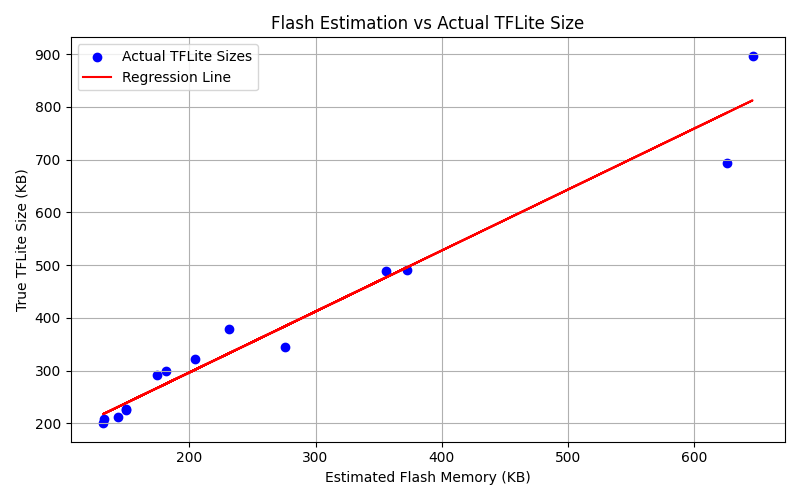
\includegraphics[width=0.85\textwidth]{Pictures/flash_regression_plot.png}
  \caption{Linear regression fit between estimated and true TFLite flash sizes.}
  \label{fig:flash-regression}
\end{figure}


Although the sample-based estimation is generally close to the actual deployment behavior, in cases where a model approaches the Flash memory limits, it is advisable to perform an early conversion to the \texttt{.tflite} format. This allows verification that the model fits within the memory constraints before proceeding with full training. The workflow consists of first converting the untrained Keras model to a TFLite version to ensure feasibility, then continuing with the regular training of the original Keras model, followed by conversion and deployment as usual.

Although this process introduces a small time overhead—typically just a few seconds—it is negligible compared to the cost of fully training a model, which can take around 20 minutes, only to later discover it cannot be deployed due to memory constraints. Conducting an early Flash feasibility check thus serves as a valuable safeguard, helping to avoid unnecessary training and conserve computational resources..

\clearpage

\subsection{Ram Memory Estimation}

During inference, each layer produces intermediate activation tensors that occupy RAM. However, not all intermediate tensors exist in memory at once – their lifetimes are limited to when they are being computed and used. A naïve approach (not reusing any buffer) would allocate a separate buffer for every intermediate tensor but this can lead to a huge memory footprint. \cite{tensorflow_RamEstimation} 


The key insight is that we can estimate the peak RAM usage by analyzing the sizes of activation tensors and understanding which ones coexist at runtime. Typically, the peak memory occurs at a layer where the largest combination of activations must be stored simultaneously. For sequential models (simple chains), this often boils down to the input and output of a single layer – once a layer’s output is produced, the previous activations can be released. \cite{liberis2019neural}

 A simplified but effective heuristic is to assume that the input and output tensors of each layer represent the concurrent memory needed during the computation of that layer, and take the maximum over all layers \cite{tensorflow_RamEstimation}. 

However, layers such as Concatenate introduce memory persistence, requiring previous activations to remain allocated until the merge operation completes. This forces multiple tensors to coexist in memory simultaneously, leading to overlapping memory demands. As a result, the real peak RAM usage can substantially exceed the simple input-output memory estimation.




As illustrated in Figure~\ref{fig:TakuNet}, our model architecture is organized into three main stages:

\begin{itemize}
    \item \textbf{Stem Block}
    \item \textbf{TakuStages Block}
    \item \textbf{Refiner Block}
\end{itemize}

The \textbf{Stem Block} and \textbf{Refiner Block} consist of consecutive layers without any additions or skip connections. Consequently, estimating the peak RAM usage for these blocks is straightforward—it corresponds to the maximum RAM required by any single layer within the block.

In contrast, each \textbf{TakuStage} includes residual operations, which require special consideration in memory estimation. Specifically, when performing concatenation or skip-connection, all input tensors must be available in memory at the same time to compute the output. This increases the peak memory footprint compared to purely sequential operations. To accurately account for this, we compute the peak RAM usage for each \textit{TakuStage} by identifying the maximum cumulative memory required across all active feature maps at any point in time. Let \( A_i \) denote the activation size of layer \( i \), and let \( \text{Live}(t) \) represent the set of layers whose outputs must remain in memory at time step \( t \). Then, the maximum RAM usage is given by:

\[
\text{MaxRAM} = \max_{t} \left( \sum_{i \in \text{Live}(t)} A_i \right)
\]

where
\[
\text{Live}(t) = \left\{ i \mid \text{output of layer } i \text{ is still needed for a future operation at time } t \right\}
\]

This formulation ensures that memory is only released after all dependencies have consumed the relevant activations.


To estimate the total maximum RAM required by the entire model, we take the maximum RAM usage from each of the three blocks and select the largest among them:

\begin{equation}
\text{RAM}_{\text{max}} = \max\left( \text{RAM}_{\text{Stem}},\ \text{RAM}_{\text{TakuStages}},\ \text{RAM}_{\text{Refiner}} \right)
\label{eq:max_ram}
\end{equation}

While the RAM estimation aligns closely with the actual measured RAM, it still tends to underestimate total memory usage due to the aforementioned memory persistence effects.

To better capture this discrepancy, we applied a similar approach as in  Section~\ref{subsec:flash_memory_estimation}, creating a linear regression model between the Estimated and Measured RAM values. The resulting line—referred to as \textit{LinearRAM}—reveals a consistent pattern in the mismatch, suggesting that a correction factor can be reliably modeled.

\begin{figure}[ht]
  \centering
  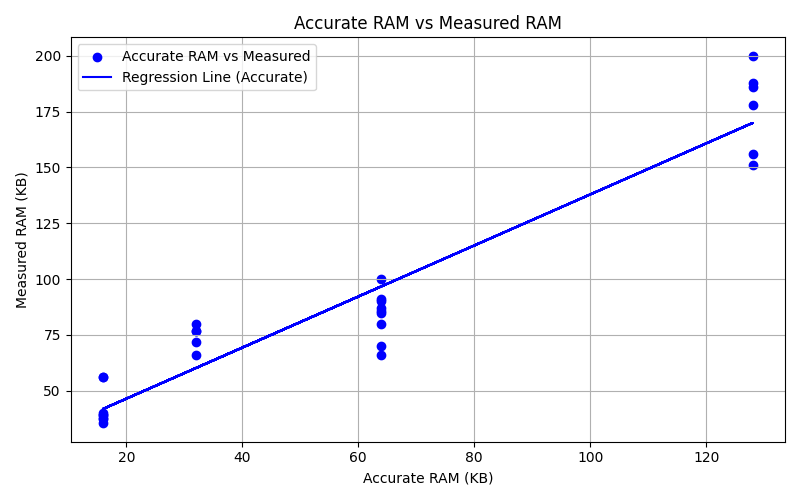
\includegraphics[width=0.85\textwidth]{Pictures/ram_accurate_vs_measured.png}
  \caption{Linear regression fit between estimated and true RAM consumption.}
  \label{fig:ram-linear-regression}
\end{figure}

\subsection{Energy Consumption Estimation}

Energy estimation is one of the most important aspects when deploying neural networks on microcontrollers, especially in power-constrained environments. The total energy consumed during a single inference can be expressed as:

\[
E = V \cdot \sum_{t=0}^{t_m} I(t) \cdot \Delta t
\]

where \( E \) is the energy in joules, \( V \) is the supply voltage (assumed constant), \( I(t) \) is the instantaneous current at time \( t \), and \( t_m \) is the duration of the inference.

In this work, the supply voltage was fixed at 3.3\,V using the Power Profiler Kit II. Figure~\ref{fig:current_profile} shows the measured current profile during a sequence of inference operations on the Arduino Nano BLE 33 Sense.

\begin{figure}[H]
    \centering
    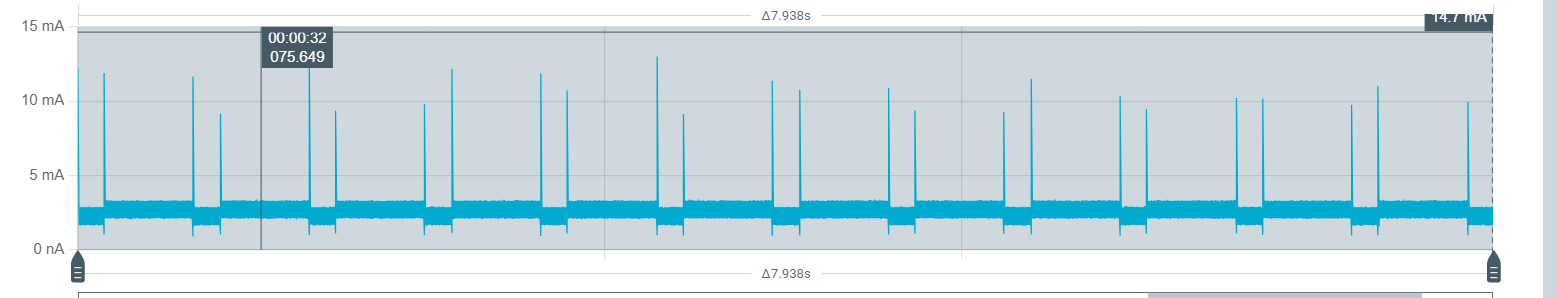
\includegraphics[width=\textwidth]{Pictures/Current.png}
    \caption{The current consumption observed during repeated model inference operations, with peaks corresponding to the active computation phases.}
    \label{fig:current_profile}
\end{figure}

As illustrated, the current remains relatively low during idle periods and exhibits distinct peaks during inference, where the processor becomes active. These peaks typically reach values around 10–15\,mA, while the baseline current hovers around 3–4\,mA.

This behavior reflects the nature of the microcontroller's operation: the Cortex-M4 CPU periodically wakes from low-power states to execute inference computations, then returns to idle. The CPU frequency—typically around 64\,MHz on the Arduino Nano BLE 33 Sense—determines how fast each instruction is executed. A higher frequency means that computations are completed faster, but it also implies more switching activity in the silicon, which increases instantaneous current draw.

However, our measurements show that the peak current is mostly determined by the processor architecture and workload type, and not by the specific neural network model. Consequently, the current profile \( I(t) \) remains relatively unchanged between models. The main variable that affects energy consumption is the inference time \( t_m \), which varies depending on the model's size and complexity.

Therefore, minimizing inference time directly contributes to energy savings, making it a key optimization objective in resource-constrained embedded AI applications.



\subsection{Inference Time Estimation}

Inference time refers to the duration a trained model requires to process an input and produce an output — essentially, the latency of a single forward-pass computation. In the context of embedded systems, inference time is a key metric, as it directly impacts both the responsiveness and energy consumption of a deployed model.

One important observation is that inference time is strongly influenced by the model’s memory (RAM) usage. 

On microcontrollers, where memory and computational bandwidth are both constrained, models that consume more RAM typically involve larger weight matrices or more extensive intermediate tensor storage. These factors increase the volume of memory access operations and place greater demand on the processor, resulting in longer inference durations.

Studies confirm that optimizing memory usage tends to speed up inference. For example, using fused in-place operations to reduce peak RAM footprint by about 1.6 × yielded a 1.2–2× faster inference execution in a TinyML context \cite{inferenceTime1}. Similarly, an embedded ML framework that lowered memory usage by 31\% achieved a remarkable 92\% reduction in inference latency compared to a less memory-efficient baseline~\cite{inferenceTime1}.


Those assumptions were confirmed after our test, finding a Linear corelation between the actual Measured RAM of the model and the inference time needed to produce the result.

\begin{figure}[ht]
  \centering
  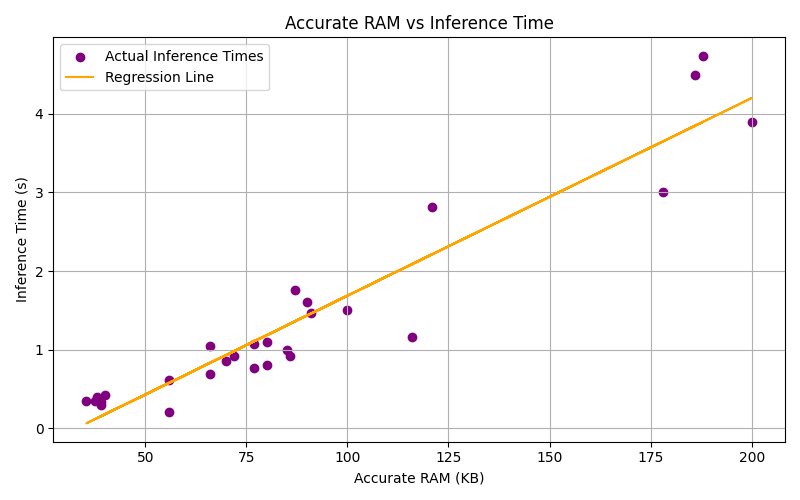
\includegraphics[width=0.85\textwidth]{Pictures/inference_time_regression_plot.png}
  \caption{Linear Corelation between RAM and Ιnference time.}
  \label{fig:inference time}
\end{figure}





\section{Selection Strategies: Tournament Selection and RankNet}

Once new models are generated in each generation of the Genetic Algorithm (GA), a critical step follows: determining which models should be selected as parents for the next generation. This selection process directly impacts the algorithm’s ability to converge efficiently toward optimal solutions, while avoiding pitfalls such as premature convergence or stagnation.

In this section, we examine two approaches designed to address this challenge: Tournament Selection, a traditional yet effective evolutionary strategy, and RankNet, a neural network-based ranking model. Each method tackles the problem of model evaluation and selection from a different perspective—one prioritizing simplicity and diversity preservation, the other aiming to accelerate selection through learned preference prediction. Their roles, mechanisms, and trade-offs are discussed in detail below.

\subsection{Tournament Selection}
Tournament Selection (TS) is a commonly used genetic selection operator in evolutionary algorithms. It addresses the fundamental challenge of balancing selective pressure toward high-fitness individuals with the maintenance of population diversity, which is crucial for avoiding premature convergence.

In TS, a small subset of individuals is chosen uniformly at random from the population, and the fittest among them is selected as a parent \cite{hussain2020trade}. This process is repeated until the desired number of parents is selected. The number of individuals in each group, known as the tournament size \textit{k}, directly controls the selection pressure: a larger \textit{k} favors the fittest individuals more strongly, while a smaller \textit{k} introduces more randomness and promotes diversity.

Unlike elitist strategies that always select the top-performing individuals, TS introduces a probabilistic component. Occasionally, sub-optimal individuals can win a tournament and propagate their genetic material, which helps maintain genetic diversity and encourages exploration of the solution space \cite{hussain2020trade}. This stochasticity is particularly important in avoiding overfitting and escaping local optima \cite{filipovic2003fine}.

Moreover, TS is computationally efficient and highly amenable to parallelization. It does not require sorting or cumulative fitness calculations, making it attractive for large-scale or real-time applications.

By maintaining a diverse gene pool and enabling exploration across multiple promising regions of the search space, TS helps evolutionary algorithms discover robust and generalizable solutions. In the context of neural architecture search, this translates to architectures that generalize better across datasets and tasks, rather than overfitting to a single performance metric.





\subsection{RankNet}

In our initial approach, we fully trained all candidate models before applying Tournament Selection (TS) to compare their performance. The top-performing models were then selected to form the next generation. However, through experimentation, we observed that this strategy was highly time-consuming, particularly because a large number of models were eventually discarded after evaluation. This inefficiency motivated us to introduce \textbf{RankNet}, a predictive model designed to estimate the relative performance of candidate architectures without requiring any training. By leveraging RankNet, we aimed to accelerate the selection process by prioritizing the most promising models early on, thus significantly reducing computational overhead.

\textbf{RankNet} is a pairwise ranking model originally developed for learning-to-rank tasks (e.g. search result ranking). It uses a shared neural network to map each input (here, an architecture embedding) to a score, then models the probability that one item is better than another by a sigmoid on the score difference \cite{RankNet}.

A key enabler for RankNet in NAS is a fixed-length embedding of each architecture that captures its structure. Recent works use graph-based embeddings; for example, Graph2Vec treats a neural network’s computational DAG as a “document” of rooted subgraphs (analogous to words) and learns a vector representation such that architectures with similar subgraph patterns are mapped close together in embedding space \cite{RankNet}.

Unlike graph-based embedding methods such as \textit{Graph2Vec}, which represent neural architectures as graphs and require complex graph encoders to learn latent representations, our approach utilizes a \textbf{lightweight, handcrafted embedding} specifically tailored to our NAS search space. This decision was motivated by the need for interpretability, computational efficiency, and tight integration with predictive models such as RankNet.

Each architecture is represented as a fixed-size vector constructed from structured, normalized parameters extracted directly from its configuration. The embedding comprises:

\begin{itemize}
    \item \textbf{Normalized architectural hyperparameters}, including:
    \begin{itemize}
        \item The number of filters, kernel sizes, and strides from the convolutional and depthwise convolutional layers across the stem, stages, and refiner blocks.
        \item The number of stages and blocks, controlling the architecture’s depth and granularity.
        \item Downsampling parameters such as pooling size and stride, which influence spatial resolution.
    \end{itemize}
    \item \textbf{One-hot encoded optimizer choices} (SGD or AdamW), allowing the model to also capture training-related configurations. This enables RankNet to infer which optimizer might better suit the architecture or dataset.
\end{itemize}

All numerical features are normalized to ensure that they lie on similar scales, improving the learning behavior of the predictive model. While simpler than graph-based embeddings, this handcrafted vector (of length 15) effectively captures both structural and training-related characteristics. It provides RankNet with a compact yet expressive input for estimating the relative performance of candidate architectures, without requiring full model training or complex processing.

Once the models are embedded, a RankNet model is trained on a set of fully evaluated networks. Rather than regressing absolute accuracy values, RankNet learns to predict *relative* performance: given a pair of architecture embeddings, it estimates the probability that one outperforms the other. The model itself uses a shared 3-layer MLP (64 $\rightarrow$ 32 $\rightarrow$ 16 units) to process each architecture embedding. A sigmoid output predicts the probability that one model outperforms another, given their embedding difference:
\begin{equation}
    P(x_i \succ x_j) = \sigma(f(x_i) - f(x_j)),
\end{equation}

where $f(x)$ is the shared MLP's score for embedding $x$. Training uses binary cross-entropy loss on pairs of fully evaluated models.This strategy is advantageous because modeling relative fitness is often more robust
and data efficient than predicting absolute scores.


To avoid computational overhead and ensure fair comparison across runs, we train RankNet only once using the fully evaluated models from the \textbf{initial population}. This snapshot provides diverse training signals while ensuring consistency.

\begin{enumerate}
    \item \textbf{One-Time Training:} RankNet is trained only once at the beginning of the search process. This decision is primarily driven by efficiency: repeated retraining would introduce significant computational overhead. By limiting training to a single round on the initial population, we reduce runtime while still providing useful ranking guidance.

    \item \textbf{Active Correction:} During tournament selection, if RankNet favors an untrained model over a trained one, we train the untrained model and compare their true performance. If RankNet’s prediction was incorrect, we retain the better-performing model and use the misprediction as a penalty signal for RankNet—effectively updating its training data to reflect this mistake in the next retraining cycle.
\end{enumerate}

Although RankNet requires pairwise comparisons to learn, it does not demand a large number of individual models. Even with a relatively small initial population (e.g., 6-10 models), we can generate a quadratic number of pairs (up to $O(n^2)$), greatly expanding the effective size of our training dataset. In our implementation, we construct \textbf{all possible pairs} from the initial population. This step is computationally cheap and does not introduce any noticeable latency in the training pipeline.

\paragraph{Pair Generation Algorithm :}
Let $x$ be the number of fully evaluated models in the initial population. The total number of unique unordered model pairs that can be generated is:

\[
\text{Number of Pairs} = \binom{x}{2} = \frac{x(x - 1)}{2}
\]

This approach enables RankNet to learn from a rich set of comparisons, even when the initial number of fully trained models is relatively small. By generating all possible pairs, we achieve data-efficient training without introducing computational overhead. In doing so, our design strikes a careful balance between efficiency and generalization: RankNet helps avoid the costly full training of weak candidates during selection, while preserving fair, one-time evaluation behavior that aligns with real-world deployment constraints.


\begin{comment}
    However, during the early stages of evolution, the RankNet model is not yet reliable due
to limited training data. To address this, we adopt two key strategies:
\begin{enumerate}
    \item \textbf{Progressive Refinement:} As the search progresses, we accumulate an increasing number of fully trained models. After each generation, we retrain the RankNet using the new pairwise comparisons, allowing the model to incrementally improve its ranking accuracy.
    
    \item \textbf{Active Correction:} During tournament selection, if RankNet favors an untrained model over a trained one, we train the untrained model and compare their true performance. If RankNet’s prediction was incorrect, we retain the better-performing model and use the misprediction as a penalty signal for RankNet—effectively updating its training data to reflect this mistake in the next retraining cycle.
\end{enumerate}

These mechanisms help RankNet adapt over time and increase the reliability of its predictions, ultimately leading to a more efficient and informed neural architecture search.
\end{comment}






\section{Speed-Up in Training}

After a model is selected—either from the initial population or through evolutionary selection—it must be trained to convergence to accurately assess its performance. However, given the potentially large number of candidate architectures evaluated throughout the search process, the cumulative training cost can become a significant bottleneck.

To address this challenge, we implemented a series of optimization strategies aimed at accelerating model training without substantially compromising final model quality. These strategies focus on reducing unnecessary computational overhead, shortening feedback loops within the NAS cycle, and promoting faster convergence. By streamlining the training phase, we improve the overall efficiency and scalability of the architecture search process.




\subsection{Performance STOP}
\label{sec:performance_stop}
To reduce training costs in Neural Architecture Search (NAS), we introduce two early stopping criteria based on the validation performance trajectory of candidate architectures. These rules enable the early termination of unpromising models, thereby conserving computational resources without significantly affecting selection quality..

Let \( A(t) \) denote the validation accuracy at epoch \( t \), and let \( T \) be the total number of epochs.

We define two criteria:
\begin{itemize}


 \item \textbf{Diminishing-returns rule}: Training is stopped if, within a continuous window of length \( \alpha T \) epochs (where \( \alpha \in (0,1) \)), the relative improvement in validation accuracy is less than a threshold \( \epsilon \). Formally, define a window \( [t, t+\alpha T] \), and stop training if:
  \[
  \frac{A(t+\alpha T) - A(t)}{A(t)} < \epsilon
  \]
  This rule captures cases of strongly diminishing returns, where continued training yields minimal gains. If the model has not shown meaningful progress during this window, it is reasonable to assume that the remaining training budget will have limited impact.

   \item \textbf{No-improvement rule}: Training is halted if the validation accuracy does not improve for a fixed number of consecutive epochs, denoted \( \tau \). That is, for \( \tau \) epochs:
  \[
  A(t) \leq A(t-1) \leq \dots \leq A(t-\tau)
  \]
  This acts as a safeguard for detecting early stagnation, even before the diminishing-returns window is reached.

\end{itemize}


These complementary criteria allow for the early termination of under-performing models based on either slow progress or complete stagnation. Empirical evaluations across various NAS runs with different training budgets (e.g., 30, 50, 70 epochs) revealed that this strategy consistently reduces training time without degrading the fidelity of model selection. Inspired by recent NAS literature advocating for efficient search via performance-based early stopping \cite{li2020random}, we incorporated both rules into our pipeline.

The specific values for the parameters \( \tau \), \( \alpha \), and \( \epsilon \) play a crucial role in balancing training speed-up against the risk of misranking high-performing models. Rather than selecting these values arbitrarily, we perform a thorough grid search to identify optimal configurations that offer strong trade-offs between efficiency and reliability. This empirical tuning ensures that our early stopping criteria remain robust across repeated runs with the same training budget.






\subsection{Early Stopping}
\label{sec:early_stopping}

Extensive research has shown that the early stages of training in convolutional neural networks (CNNs) play a disproportionately important role in shaping a model’s final performance. In particular, the initial epochs often establish the core representational capacity of the network and largely determine its generalization behavior.

A notable study on “critical learning periods” reports that “the first few epochs are critical for the creation of strong connections,” which “do not appear to change during additional training” \cite{achille2017critical}. The authors conclude that this early phase is central to the learning process and heavily influences the model’s final outcome. Empirically, this translates to much of a CNN’s eventual validation accuracy being attained early in training, with subsequent epochs providing only marginal improvements.

Figure~\ref{fig:val_accuracy} illustrates this phenomenon for several \texttt{TakuNet} models. The normalized validation accuracy curves reveal that:
\begin{itemize}
  \item By epoch 5 out of 30 (just \( \frac{5}{30} \times 100 = 16.7\% \) of the total training time), each model achieves approximately 70\% of its final validation accuracy.
  \item By epoch 10 (33.4\% of training), models typically reach around 80\% of their eventual performance.
\end{itemize}

These observations highlight the efficiency of early training and provide strong motivation for the use of early stopping mechanisms. More importantly, they inspired us to investigate whether models that perform poorly in the early epochs could be confidently identified and excluded from full training. This insight laid the foundation for our performance-based stopping criteria, which aim to cut short the training of under-performing architectures—saving significant computational resources without compromising the quality of the search.

To leverage this behavior in our NAS pipeline, we introduced a custom callback mechanism that monitors validation accuracy at a strategic checkpoint. If the validation accuracy fails to exceed a predefined threshold by a specific fraction of the training process, the model is deemed unpromising and its training is cut early. Formally, let \( A(t) \) denote the validation accuracy at epoch \( t \), and let \( T \) be the total number of training epochs. We define an early termination condition as:

\[
A(t) < A_{\min} \quad \text{where} \quad t = \lfloor \beta \rfloor
\]

Here, \( \beta \in (0,1) \) represents the early evaluation point (as a fraction of total training), and \( A_{\min} \) is the minimum acceptable validation accuracy at that checkpoint.

Empirical analysis across different search runs and training budgets confirmed the effectiveness of this rule in identifying weak models early. By eliminating such architectures before completing the full training cycle, we were able to substantially reduce computational overhead while preserving the quality and reliability of model selection in the NAS process.


Notably, we observed that the optimal values for the evaluation point \( \beta \) and the minimum acceptable accuracy \( A_{\min} \) depend on the total training budget. That is, different training durations (e.g., 30, 50, or 70 epochs) may require different early stopping thresholds to maintain selection reliability. However, for any given training schedule, the chosen parameters remained stable and reproducible across multiple independent NAS runs. This consistency suggests that early stopping criteria can be effectively calibrated once per training regime and then reused across searches, without the need for frequent re-tuning.




\begin{figure}[H]
    \centering
    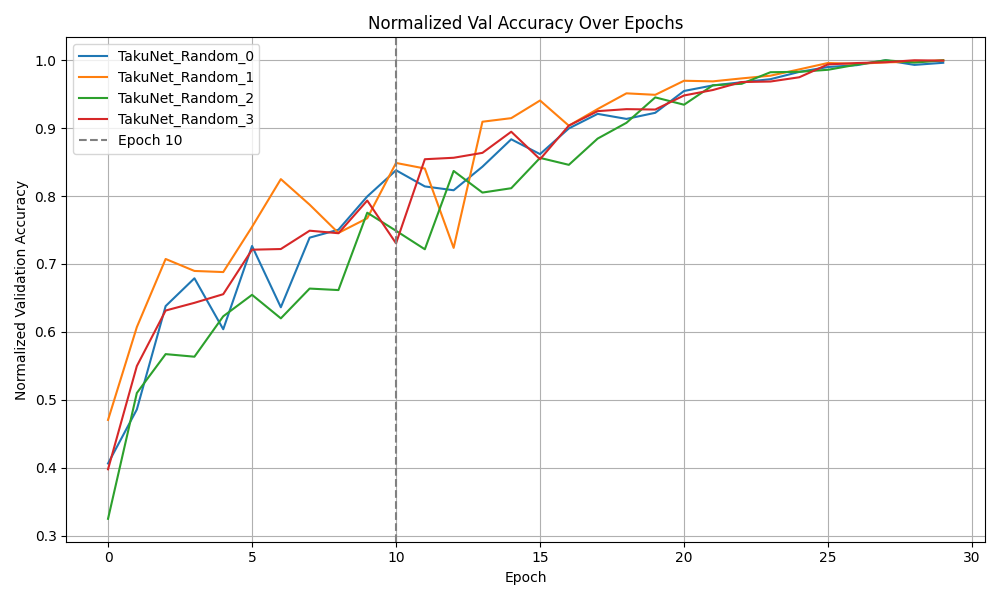
\includegraphics[width=0.85\linewidth]{Pictures/val_accuracy_comparison.png}
    \caption{Normalized validation accuracy curves for different TakuNet variants.}
    \label{fig:val_accuracy}
\end{figure}




\subsection{Learning Rate Scheduling}

One of the most important factors influencing the training dynamics of deep neural networks is the learning rate. It controls the step size taken during gradient descent and directly affects how quickly and effectively a model converges. A poorly chosen learning rate can lead to slow training, suboptimal convergence, or even complete instability. Conversely, an appropriate learning rate schedule can significantly improve both training speed and final performance.

In practice, even fixed learning rates—if well-tuned—can lead to strong results, especially when training for a large number of epochs. However, static learning rates often fail to adapt to the changing optimization landscape over time. Early in training, large updates are generally beneficial for escaping sharp minima and accelerating exploration. Later, smaller learning rates are preferable for fine-tuning and convergence.

To balance these needs, we adopted a dynamic learning rate strategy that combines a linear warm-up phase with cosine annealing. The learning rate starts from a low initial value and increases linearly over the first 5 epochs (warm-up), then gradually decays following a cosine curve relative to the total number of training epochs.

This scheduling approach, inspired by the method introduced in \cite{loshchilov2016sgdr}, helps stabilize early training and encourages smoother convergence. The cosine decay promotes better generalization by allowing the model to settle into flatter, wider optima that are less sensitive to parameter noise.


The cosine function used ,inspired by \cite{loshchilov2016sgdr} : 

\begin{equation}
\text{lr}(t) = \eta_0 \cdot \frac{1}{2} \left( 1 + \cos\left( \frac{\pi (t - T_\text{warmup})}{T_\text{total} - T_\text{warmup}} \right) \right),
\end{equation}

where:
\begin{itemize}
  \item \( \eta_0 \) is the initial learning rate,
  \item \( T_\text{warmup} \) is the number of warmup epochs,
  \item \( T_\text{total} \) is the total number of training epochs,
  \item \( t \) is the current epoch number.
\end{itemize}


Cosine learning rate schedules have been widely adopted in modern image classification models such as ResNet, DenseNet, and MobileNet, and are considered state-of-the-art for datasets like CIFAR-10 and CIFAR-100~\cite{lewkowycz2021decay}. Studies show that cosine decay leads to faster convergence and slightly improved final accuracy compared to traditional step-based schedules.

As illustrated in Figure~\ref{fig:val_accuracy_diff_epochs}, for a  random TakuNet model, increasing the number of training epochs does not significantly improve validation accuracy, given the Learning Rate Scheduling technique used. This saturation effect aligns with the theoretical behavior of cosine decay: once the learning rate approaches zero, further updates become minimal.

This observation motivated us to investigate the optimal number of training epochs that would strike a balance between maximizing speed-up and minimizing misranking error within our NAS pipeline.
To this end, we conducted a series of experiments aimed at identifying the sweet spot where training time could be significantly reduced, while still preserving high reliability in predicting which models outperform others.

\begin{figure}[ht]
    \centering
    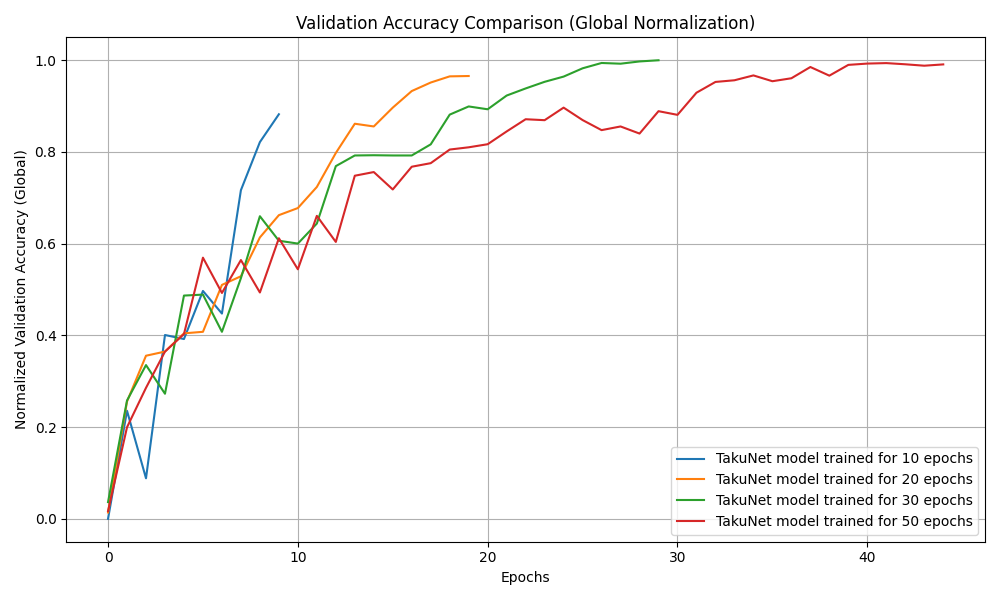
\includegraphics[width=0.85\linewidth]{Pictures/val_accuracy_comparison_global.png}
    \caption{Normalized Validation accuracy(based on highest recorder accuracy) of TakuNet trained for different number of epochs }
    \label{fig:val_accuracy_diff_epochs}
\end{figure}

\section{Post training Optimization}

% For additional technical context, consult the official guide at:
% https://ai.google.dev/edge/litert/models/post_training_quantization

In this work, the trained neural networks are converted from Keras models to TensorFlow Lite (TFLite) format using full integer quantization, enabling deployment on memory-constrained embedded devices such as the Arduino Nano BLE 33 Sense. While the original Keras models operate in 32-bit floating-point precision, the TFLite conversion process maps both weights and activations to 8-bit integers. This reduction in numerical precision can, in theory, lead to minor accuracy degradation.

Quantization may introduce rounding errors in arithmetic operations and discretization effects during inference, especially near activation boundaries. Furthermore, optimized TFLite kernels for layers such as depthwise convolutions or batch normalization may behave slightly differently from their float32 counterparts in Keras. These differences, though usually subtle, can affect model outputs.

To mitigate such effects and preserve the model's predictive performance, we follow the post-training quantization procedure recommended by Google’s official guidelines~\cite{tensorflow2023quantization}. Specifically, we supply a representative dataset during the quantization step. This dataset, drawn from the same distribution as the training and validation data, is used to calibrate the dynamic range of the activations, ensuring that the int8 quantized model accurately reflects the statistical properties of the original float32 model.

Using this method, we aimed to ensure that the accuracy of the quantized TFLite model remains equivalent to that of its original float32 counterpart. As a result, we are able to safely omit re-evaluating the model's accuracy on the embedded device itself, thus saving time during deployment. Instead, we rely on the model's validation accuracy prior to quantization for performance comparisons, assuming that the post-quantization accuracy loss is negligible—as confirmed both by our empirical results and the recommended quantization procedure.